%
% File: chap02.tex
%
\let\textcircled=\pgftextcircled
\chapter{Proposed solution (Graph Partitioning for Large Graphs)}
\label{Chapter3}
GNNs aim at learning node
representations by learning the similarities shared between
connected nodes. However, the expressive ability of a GNN
is highly dependent on the quality of node features
Mention here: Deep Fraud Detection on Non-attributed Graph
https://arxiv.org/pdf/2110.01171.pdf
but cited here
C. T. Duong, T. D. Hoang, H. T. H. Dang, Q. V. H. Nguyen, and
K. Aberer, “On node features for graph neural networks,” arXiv preprint
arXiv:1911.08795, 2019.
[11] H. Cui, Z. Lu, P. Li, and C. Yang, “On positional and structural node
features for graph neural networks on non-attributed graphs,” arXiv
preprint arXiv:2107.01495, 2021

Eigendecomposition and top-k-eigenvalues are the k-dimensional feature vector
Q. Huang, H. He, A. Singh, S.-N. Lim, and A. R. Benson, “Combining
label propagation and simple models out-performs graph neural net-
works,” arXiv preprint arXiv:2010.13993, 2020.

Different feature initializations
http://www.cs.emory.edu/~jyang71/files/gnnfeature.pdf

\begin{center}
    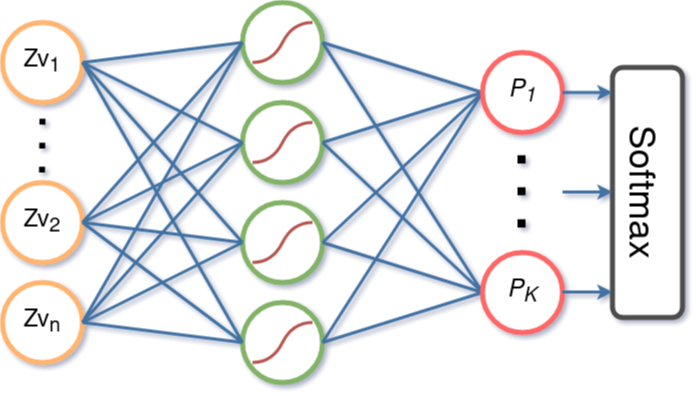
\includegraphics[scale=0.5]{partitioning_module}
\end{center}

One of the principal limitations that GAP has is that it requires 

According to the original paper~\cite{deepwalk}, the DeepWalk algorithm consists of two main components: a random walk generator and an update procedure. 

In the first component, a random node $v_i$ is taken uniformly at random to be the root of a random walk $\mathcal W_{v_i}$ which in its turn samples recursively from the neighbors of the last visited vertex until the maximum length $\gamma$ is reached.

As specified by Perozzi et. al.~\citep{deepwalk}, their experiments suggest that the number of walks started per vertex should be greater or equal than $\gamma=30$, the latent dimension greater or equal than $d=64$, and they fixed the sensible values of $w=10$ for the window size, and $t=40$ for the walk length . Based on those recommendations, in the experiments carried out in~\citep{deepwalk_hyper}, and the computational needs of the problem to be solver, it was found convenient to set $\gamma=60$, $d=64$, $w=10$(good results with 15), and $t=60$ (good results with 80).


For the algorithm that is proposed here, the implementation by the Karate Club API~\cite{karateclub} was used.